\chapter{Thiết kế Cơ sở dữ liệu Logic và Chuẩn hóa}

Trong chương này, dự án sẽ tiến hành chuyển đổi từ mô hình thực thể quan niệm (ERD) sang lược đồ cơ sở dữ liệu quan hệ (Logic). Quá trình này được thực hiện thông qua các thuật toán ánh xạ, sau đó áp dụng lý thuyết phụ thuộc hàm để chứng minh các lược đồ đạt dạng chuẩn Boyce-Codd (BCNF), đảm bảo tính toàn vẹn dữ liệu và tối ưu hóa lưu trữ trước khi chuyển sang thiết kế vật lý.

\section{Chuyển đổi từ Mô hình Quan niệm sang Lược đồ Logic}

Dựa trên sơ đồ thực thể kết hợp (ERD) và các quy tắc nghiệp vụ đã phân tích ở Chương 2, tiến hành chuyển đổi mô hình thực thể quan niệm sang mô hình quan hệ (Relational Schema). Quá trình chuyển đổi được thực hiện thông qua các quy tắc ánh xạ từ ER sang quan hệ nhằm bảo đảm các thực thể, thuộc tính, khóa và mối kết hợp trong mô hình logic phù hợp với mô hình quan niệm.

\subsection{Các quy tắc chuyển đổi áp dụng}

Quá trình ánh xạ từ ERD sang Lược đồ Logic tuân thủ các quy tắc cốt lõi sau:

\begin{itemize}
    \item \textbf{Quy tắc 1 (Ánh xạ thực thể mạnh):} 
    Mỗi thực thể mạnh trong ERD được chuyển thành một quan hệ (bảng). 
    Các thuộc tính của thực thể trở thành các thuộc tính của quan hệ và khóa định danh của thực thể trở thành khóa chính (Primary Key - PK).

    \item \textbf{Quy tắc 2 (Ánh xạ mối kết hợp 1:N):} 
    Đối với mối kết hợp một-nhiều (1:N), khóa chính của thực thể phía ``1'' được đưa sang thực thể phía ``N'' làm khóa ngoại (Foreign Key - FK).
    
    Ví dụ, \texttt{TENANT} có nhiều \texttt{MERCHANT}, do đó \texttt{TenantID} được đặt trong bảng \texttt{MERCHANT} làm khóa ngoại.

    \item \textbf{Quy tắc 3 (Ánh xạ mối kết hợp M:N):} 
    Đối với mối kết hợp nhiều-nhiều (M:N), tạo một quan hệ trung gian chứa khóa của hai thực thể tham gia.
    
    Trong mô hình OctaPoint, mối kết hợp giữa \texttt{CAMPAIGN} và \texttt{MERCHANT} được phân rã thông qua bảng \texttt{CAMPAIGN\_MERCHANT}. Hai thuộc tính \texttt{CampaignID} và \texttt{MerchantID} đồng thời là khóa ngoại và tạo thành khóa chính ghép của quan hệ trung gian.

    \item \textbf{Quy tắc 4 (Ánh xạ quan hệ CREDIT):}
    \texttt{CREDIT} biểu diễn ví điểm dùng chung của một \texttt{CUSTOMER} trong phạm vi một \texttt{TENANT}. Vì vậy, bảng \texttt{CREDIT} chứa \texttt{CustomerID} và \texttt{TenantID}. 
    Để bảo đảm mỗi khách hàng chỉ có tối đa một ví điểm trong một Tenant, áp dụng ràng buộc \texttt{UNIQUE(CustomerID, TenantID)}.

    \item \textbf{Quy tắc 5 (Quan hệ tự tham chiếu):}
    Quan hệ quản lý nhân sự trong \texttt{USER} được ánh xạ bằng thuộc tính \texttt{ManagerID}. Thuộc tính này là khóa ngoại tham chiếu đến \texttt{UserID} của chính bảng \texttt{USER} và cho phép giá trị NULL đối với người không có người quản lý trực tiếp.

    \item \textbf{Quy tắc 6 (Giao dịch điểm):}
    \texttt{CREDIT\_TRANSACTION} tham chiếu đến \texttt{CREDIT} và \texttt{MERCHANT}. 
    \texttt{CampaignID} được phép NULL vì một giao dịch điểm có thể phát sinh mà không gắn với một chiến dịch cụ thể.
\end{itemize}

\subsection{Danh sách Lược đồ Quan hệ}

Dựa trên ERD của OctaPoint CaaS, tập hợp các lược đồ quan hệ được xác định như sau. Quy ước: thuộc tính gạch chân là Khóa chính (PK), thuộc tính in nghiêng là Khóa ngoại (FK).

\begin{description}

    \item[\texttt{TENANT}]
    (\underline{TenantID}, TenantName)

    \item[\texttt{MERCHANT}]
    (\underline{MerchantID}, \textit{TenantID}, BusinessName, Status)

    \item[\texttt{ROLE}]
    (\underline{RoleID}, RoleName)

    \item[\texttt{USER}]
    (\underline{UserID}, \textit{RoleID}, \textit{ManagerID}, \textit{MerchantID}, Email, PasswordHash)

    \item[\texttt{CUSTOMER}]
    (\underline{CustomerID}, Email, WalletAddress)

    \item[\texttt{CREDIT}]
    (\underline{CreditID}, \textit{CustomerID}, \textit{TenantID}, AvailableBalance)

    \item[\texttt{CAMPAIGN}]
    (\underline{CampaignID}, \textit{TenantID}, Status, StartDate)

    \item[\texttt{CAMPAIGN\_MERCHANT}]
    (\underline{\textit{CampaignID}}, \underline{\textit{MerchantID}})

    \item[\texttt{REWARD\_RULE}]
    (\underline{RuleID}, \textit{CampaignID}, ActionType, PointsMultiplier)

    \item[\texttt{CREDIT\_TRANSACTION}]
    (\underline{TransactionID}, \textit{CreditID}, \textit{MerchantID}, \textit{CampaignID}, Amount, CreatedAt, TransactionType, SuiTxDigest)

    \item[\texttt{API\_CREDENTIAL}]
    (\underline{KeyID}, \textit{MerchantID}, ApiKey, SecretHash)

\end{description}

\section{Phụ thuộc hàm và Khóa ứng viên}

Phân tích phụ thuộc hàm được thực hiện riêng trên từng quan hệ. Các thuộc tính cùng tên ở những quan hệ khác nhau được xem là các thuộc tính thuộc các quan hệ riêng biệt. Kết luận chuẩn hóa được xây dựng dựa trên tập phụ thuộc hàm nghiệp vụ được xác định trong mô hình logic.

\subsection{Tập phụ thuộc hàm được xét}

Ký hiệu $R$ là tập toàn bộ thuộc tính của quan hệ tương ứng. Các phụ thuộc hàm được xét như sau:

\begin{itemize}

    \item \textbf{TENANT:}
    \[
    TenantID \rightarrow R
    \]

    \item \textbf{MERCHANT:}
    \[
    MerchantID \rightarrow R
    \]

    \item \textbf{ROLE:}
    \[
    RoleID \rightarrow R
    \]

    \item \textbf{USER:}
    \[
    UserID \rightarrow R
    \]
    \[
    Email \rightarrow R
    \]
    với $R$ gồm:
    \[
    \{UserID, RoleID, ManagerID, MerchantID, Email, PasswordHash\}
    \]

    \item \textbf{CUSTOMER:}
    \[
    CustomerID \rightarrow R
    \]

    \item \textbf{CREDIT:}
    \[
    CreditID \rightarrow R
    \]
    \[
    (CustomerID,TenantID) \rightarrow R
    \]

    \item \textbf{CAMPAIGN:}
    \[
    CampaignID \rightarrow R
    \]

    \item \textbf{CAMPAIGN\_MERCHANT:}
    \[
    (CampaignID,MerchantID) \rightarrow R
    \]

    \item \textbf{REWARD\_RULE:}
    \[
    RuleID \rightarrow R
    \]

    \item \textbf{CREDIT\_TRANSACTION:}
    \[
    TransactionID \rightarrow R
    \]

    \item \textbf{API\_CREDENTIAL:}
    \[
    KeyID \rightarrow R
    \]
    \[
    ApiKey \rightarrow R
    \]

\end{itemize}

Trong đó, \texttt{Email} của \texttt{USER} và \texttt{ApiKey} của \texttt{API\_CREDENTIAL} được xác định là các thuộc tính duy nhất và không NULL.
Đối với bảng \texttt{CREDIT}, cặp $(CustomerID,TenantID)$ là khóa nghiệp vụ duy nhất. Một khách hàng có thể tham gia nhiều Tenant khác nhau, nhưng trong cùng một Tenant chỉ có tối đa một Credit tương ứng.
Không giả định các thuộc tính như \texttt{RoleName}, \texttt{Customer.Email}, \texttt{Status}, \texttt{ActionType} hoặc các thuộc tính mô tả khác là khóa nếu chưa có ràng buộc UNIQUE tương ứng.

\subsection{Bao đóng và tính tối thiểu}
\subsubsection{Quan hệ USER}
Với khóa \texttt{UserID}:

\[
\{UserID\}^{+}=R_{USER}
\]

Do đó, \texttt{UserID} là khóa ứng viên.
Với \texttt{Email}:

\[
\{Email\}^{+}=R_{USER}
\]

Do \texttt{Email} được quy định là UNIQUE và NOT NULL, \texttt{Email} cũng là một khóa ứng viên của quan hệ \texttt{USER}.
Vì vậy, các khóa ứng viên của \texttt{USER} là:

\[
\{UserID\},\{Email\}
\]

\subsubsection{Quan hệ CREDIT}

Với \texttt{CreditID}:

\[
\{CreditID\}^{+}=R_{CREDIT}
\]

Do đó, \texttt{CreditID} là khóa ứng viên.
Với cặp $(CustomerID,TenantID)$:

\[
\{CustomerID,TenantID\}^{+}=R_{CREDIT}
\]

Do đó:

\[
(CustomerID,TenantID)
\]

là khóa ứng viên thứ hai.

\texttt{CustomerID} riêng lẻ không xác định được một Credit duy nhất vì một khách hàng có thể có Credit tại nhiều Tenant.
Tương tự, \texttt{TenantID} riêng lẻ không xác định được một Credit duy nhất vì một Tenant có thể có nhiều khách hàng.
Vì vậy, khóa nghiệp vụ tối thiểu của \texttt{CREDIT} là:

\[
\{CustomerID,TenantID\}
\]

Trong triển khai, \texttt{CreditID} được chọn làm khóa chính để các giao dịch tham chiếu đến Credit thuận tiện hơn. Đồng thời, ràng buộc:

\[
UNIQUE(CustomerID,TenantID)
\]

được duy trì để bảo đảm tính duy nhất theo nghiệp vụ.

\subsubsection{Quan hệ API\_CREDENTIAL}

Với \texttt{KeyID}:

\[
\{KeyID\}^{+}=R_{API\_CREDENTIAL}
\]

Với \texttt{ApiKey}:

\[
\{ApiKey\}^{+}=R_{API\_CREDENTIAL}
\]

Do đó, hai khóa ứng viên của quan hệ \texttt{API\_CREDENTIAL} là:

\[
\{KeyID\},\{ApiKey\}
\]

\subsubsection{Các quan hệ còn lại}
Đối với \texttt{TENANT}, \texttt{MERCHANT}, \texttt{ROLE}, \texttt{CUSTOMER}, \texttt{CAMPAIGN}, \texttt{REWARD\_RULE} và \texttt{CREDIT\_TRANSACTION}, khóa định danh của mỗi quan hệ có bao đóng bằng toàn bộ tập thuộc tính của quan hệ tương ứng.
Do đó, các khóa ứng viên lần lượt là:

\[
TenantID
\]

\[
MerchantID
\]

\[
RoleID
\]

\[
CustomerID
\]

\[
CampaignID
\]

\[
RuleID
\]

\[
TransactionID
\]

Đối với \texttt{CAMPAIGN\_MERCHANT}, khóa chính ghép là:

\[
(CampaignID,MerchantID)
\]

Hai thuộc tính riêng lẻ không xác định được toàn bộ quan hệ vì một Campaign có thể áp dụng cho nhiều Merchant và một Merchant có thể tham gia nhiều Campaign.

\section{Chuẩn hóa Dữ liệu}

Một quan hệ đạt BCNF nếu với mọi phụ thuộc hàm không tầm thường:
\[
X \rightarrow Y
\]
thì $X$ phải là một siêu khóa của quan hệ.
Dựa trên tập phụ thuộc hàm đã xác định, các vế trái của các phụ thuộc hàm đều là khóa ứng viên hoặc siêu khóa của quan hệ tương ứng.
Do đó, các quan hệ:

\begin{itemize}
    \item TENANT
    \item MERCHANT
    \item ROLE
    \item USER
    \item CUSTOMER
    \item CREDIT
    \item CAMPAIGN
    \item CAMPAIGN\_MERCHANT
    \item REWARD\_RULE
    \item CREDIT\_TRANSACTION
    \item API\_CREDENTIAL
\end{itemize}

đều đạt chuẩn BCNF theo tập phụ thuộc hàm được xét.
Kết quả chuẩn hóa giúp giảm dư thừa dữ liệu và các dị thường cập nhật đối với các phụ thuộc hàm đã xác định. Tuy nhiên, BCNF không thay thế các ràng buộc toàn vẹn tham chiếu, ràng buộc miền giá trị hoặc các quy tắc nghiệp vụ khác.
Đối với thuộc tính \texttt{AvailableBalance}, đây là số dư được lưu sẵn nhằm hỗ trợ truy vấn nhanh. Tính nhất quán giữa số dư và các giao dịch trong \texttt{CREDIT\_TRANSACTION} cần được bảo đảm bởi các quy tắc nghiệp vụ của hệ thống.

\subsection{Cách kiểm tra dạng chuẩn}
\textbf{Dạng chuẩn 1NF (First Normal Form):} mỗi ô dữ liệu chứa một giá trị đơn thuộc miền dữ liệu đã xác định, không chứa danh sách hoặc nhóm lặp.
\textbf{Dạng chuẩn 2NF (Second Normal Form):} quan hệ phải đạt 1NF và mọi thuộc tính không khóa phải phụ thuộc đầy đủ vào toàn bộ khóa ứng viên, không phụ thuộc vào một phần của khóa ghép.
\textbf{Dạng chuẩn 3NF (Third Normal Form):} với mỗi phụ thuộc hàm không tầm thường $X \rightarrow A$, $X$ phải là siêu khóa hoặc $A$ phải là thuộc tính khóa.
\textbf{Dạng chuẩn BCNF:} với mọi phụ thuộc hàm không tầm thường $X \rightarrow Y$, $X$ phải là siêu khóa.

Ví dụ, nếu đưa \texttt{TenantName} vào bảng \texttt{MERCHANT}, sẽ phát sinh phụ thuộc:
\[
MerchantID \rightarrow TenantID
\]
và:
\[
TenantID \rightarrow TenantName
\]
Điều này làm cho tên Tenant bị lặp lại trên nhiều dòng Merchant thuộc cùng một Tenant. Vì vậy, \texttt{TenantName} được lưu tại bảng \texttt{TENANT} và \texttt{MERCHANT} chỉ tham chiếu thông qua \texttt{TenantID}.

\section{Sơ đồ Lược đồ Logic (Logical Schema Diagram)}

Lược đồ logic được xây dựng dựa trên mô hình ERD đã hoàn thiện và tập phụ thuộc hàm được xác định ở các mục trước. Sơ đồ thể hiện các quan hệ, thuộc tính, khóa chính (Primary Key - PK), khóa ngoại (Foreign Key - FK) và bản số của các mối quan hệ.

Trong mô hình OctaPoint, \texttt{CREDIT} là ví điểm dùng chung của một \texttt{CUSTOMER} trong phạm vi một \texttt{TENANT}. Vì vậy, \texttt{CREDIT} tham chiếu đến \texttt{CUSTOMER} và \texttt{TENANT}, không tham chiếu trực tiếp đến \texttt{MERCHANT}.

Bên cạnh đó, \texttt{CAMPAIGN} thuộc về một \texttt{TENANT}. Một Campaign có thể áp dụng cho nhiều Merchant và một Merchant có thể tham gia nhiều Campaign. Do đó, mối quan hệ M:N giữa \texttt{CAMPAIGN} và \texttt{MERCHANT} được phân rã thông qua bảng trung gian \texttt{CAMPAIGN\_MERCHANT}.

\begin{figure}[H]
    \centering
    \resizebox{\textwidth}{!}{
    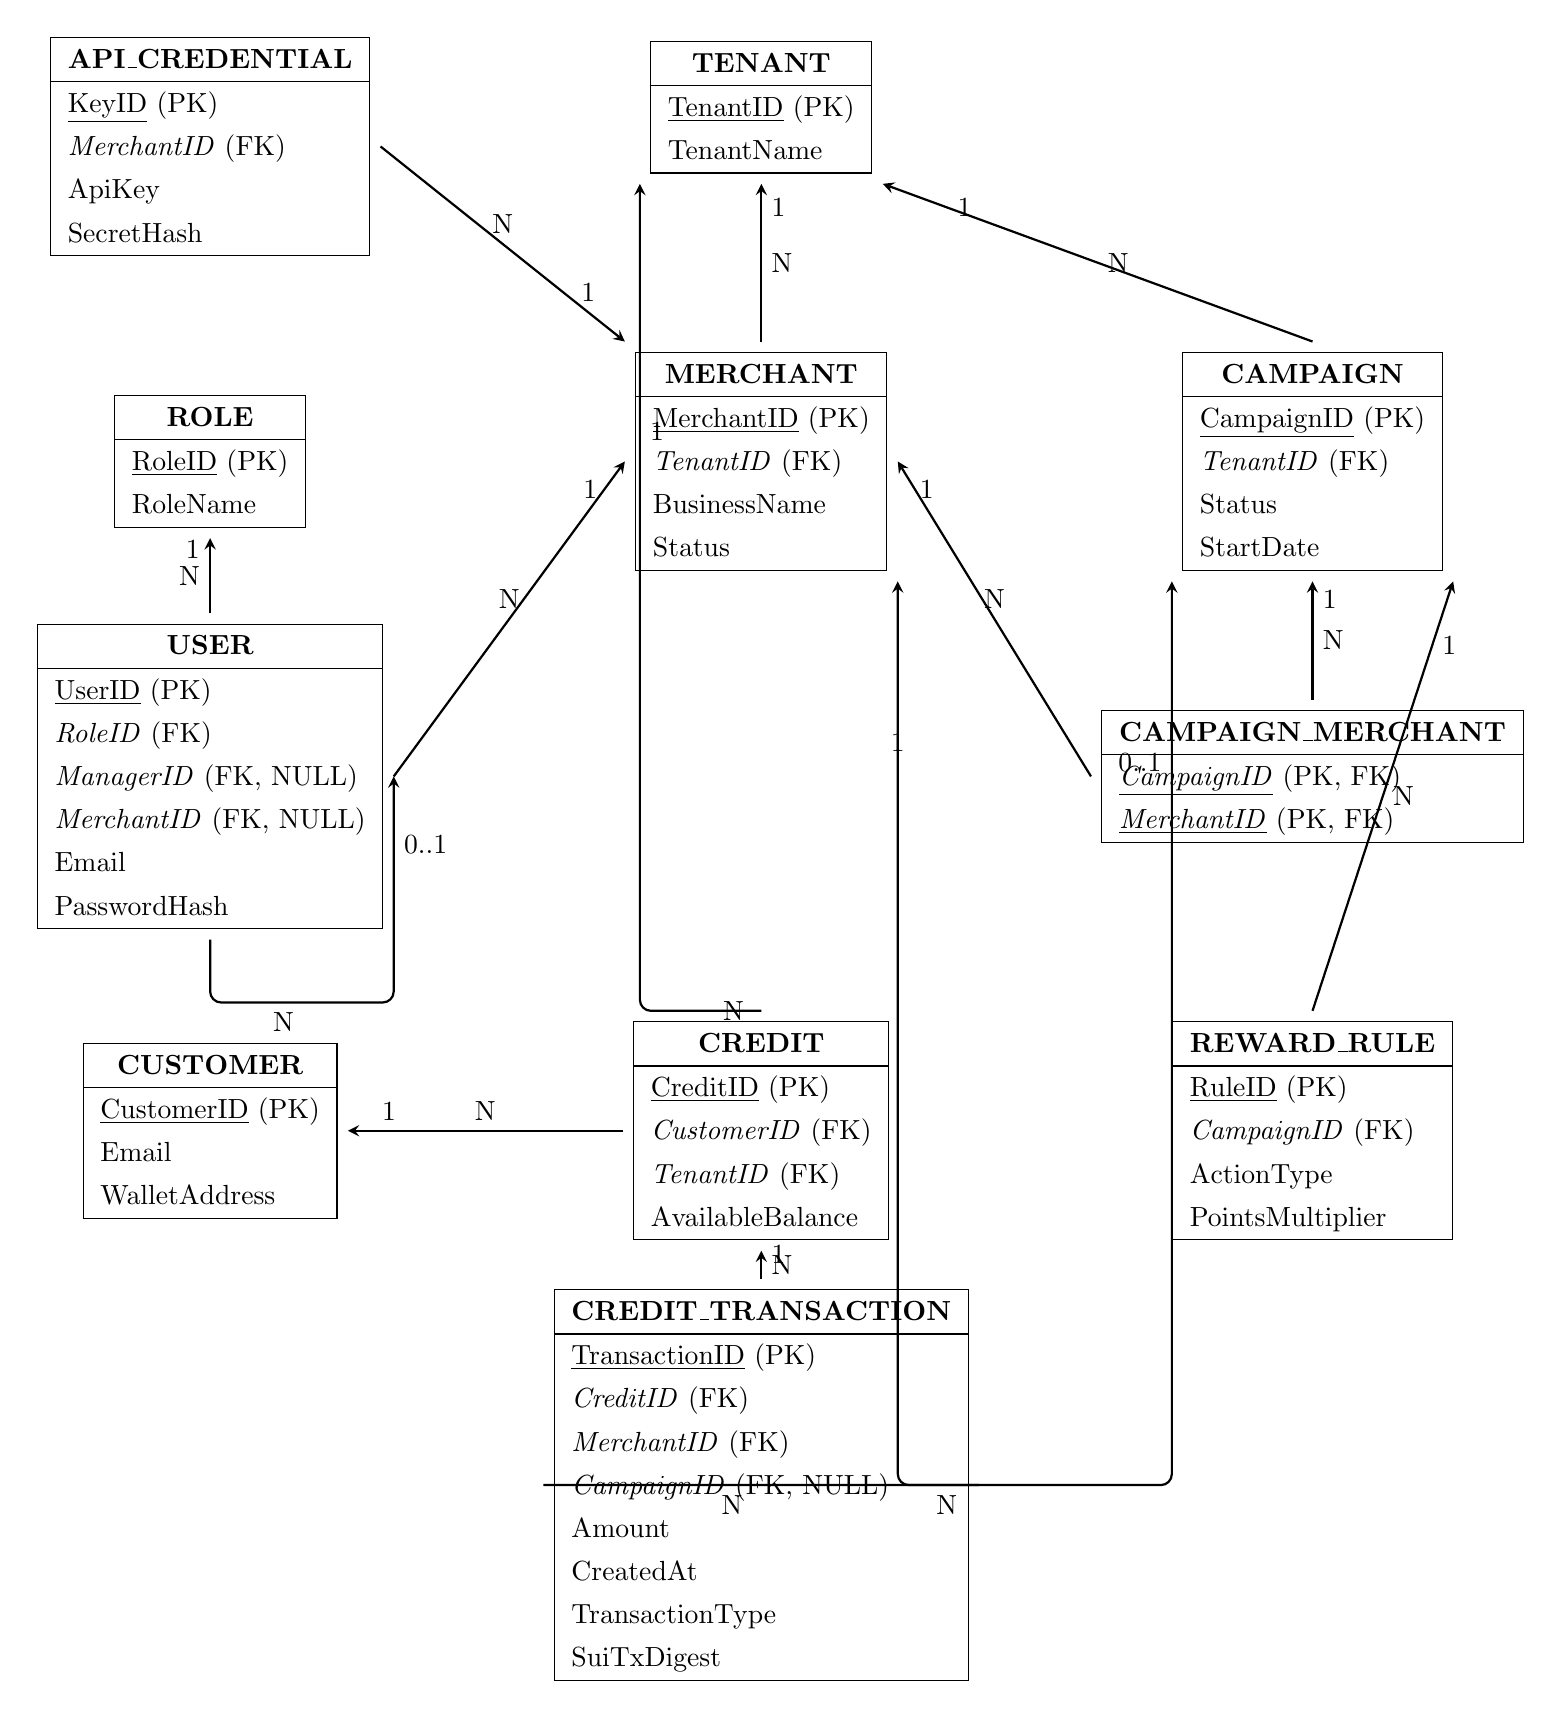
\begin{tikzpicture}[>=stealth, thick]

        % ========================================================
        % TENANT
        % ========================================================
        \node (tenant) at (0,6) {
            \begin{tabular}{|l|}
            \hline
            \multicolumn{1}{|c|}{\textbf{TENANT}} \\ \hline
            \underline{TenantID} (PK) \\
            TenantName \\ \hline
            \end{tabular}
        };

        % ========================================================
        % MERCHANT
        % ========================================================
        \node (merchant) at (0,1.5) {
            \begin{tabular}{|l|}
            \hline
            \multicolumn{1}{|c|}{\textbf{MERCHANT}} \\ \hline
            \underline{MerchantID} (PK) \\
            \textit{TenantID} (FK) \\
            BusinessName \\
            Status \\ \hline
            \end{tabular}
        };

        % ========================================================
        % ROLE
        % ========================================================
        \node (role) at (-7,1.5) {
            \begin{tabular}{|l|}
            \hline
            \multicolumn{1}{|c|}{\textbf{ROLE}} \\ \hline
            \underline{RoleID} (PK) \\
            RoleName \\ \hline
            \end{tabular}
        };

        % ========================================================
        % USER
        % ========================================================
        \node (user) at (-7,-2.5) {
            \begin{tabular}{|l|}
            \hline
            \multicolumn{1}{|c|}{\textbf{USER}} \\ \hline
            \underline{UserID} (PK) \\
            \textit{RoleID} (FK) \\
            \textit{ManagerID} (FK, NULL) \\
            \textit{MerchantID} (FK, NULL) \\
            Email \\
            PasswordHash \\ \hline
            \end{tabular}
        };

        % ========================================================
        % API CREDENTIAL
        % ========================================================
        \node (api) at (-7,5.5) {
            \begin{tabular}{|l|}
            \hline
            \multicolumn{1}{|c|}{\textbf{API\_CREDENTIAL}} \\ \hline
            \underline{KeyID} (PK) \\
            \textit{MerchantID} (FK) \\
            ApiKey \\
            SecretHash \\ \hline
            \end{tabular}
        };

        % ========================================================
        % CAMPAIGN
        % ========================================================
        \node (campaign) at (7,1.5) {
            \begin{tabular}{|l|}
            \hline
            \multicolumn{1}{|c|}{\textbf{CAMPAIGN}} \\ \hline
            \underline{CampaignID} (PK) \\
            \textit{TenantID} (FK) \\
            Status \\
            StartDate \\ \hline
            \end{tabular}
        };

        % ========================================================
        % CAMPAIGN MERCHANT
        % ========================================================
        \node (cm) at (7,-2.5) {
            \begin{tabular}{|l|}
            \hline
            \multicolumn{1}{|c|}{\textbf{CAMPAIGN\_MERCHANT}} \\ \hline
            \underline{\textit{CampaignID}} (PK, FK) \\
            \underline{\textit{MerchantID}} (PK, FK) \\ \hline
            \end{tabular}
        };

        % ========================================================
        % CUSTOMER
        % ========================================================
        \node (customer) at (-7,-7) {
            \begin{tabular}{|l|}
            \hline
            \multicolumn{1}{|c|}{\textbf{CUSTOMER}} \\ \hline
            \underline{CustomerID} (PK) \\
            Email \\
            WalletAddress \\ \hline
            \end{tabular}
        };

        % ========================================================
        % CREDIT
        % ========================================================
        \node (credit) at (0,-7) {
            \begin{tabular}{|l|}
            \hline
            \multicolumn{1}{|c|}{\textbf{CREDIT}} \\ \hline
            \underline{CreditID} (PK) \\
            \textit{CustomerID} (FK) \\
            \textit{TenantID} (FK) \\
            AvailableBalance \\ \hline
            \end{tabular}
        };

        % ========================================================
        % REWARD RULE
        % ========================================================
        \node (rule) at (7,-7) {
            \begin{tabular}{|l|}
            \hline
            \multicolumn{1}{|c|}{\textbf{REWARD\_RULE}} \\ \hline
            \underline{RuleID} (PK) \\
            \textit{CampaignID} (FK) \\
            ActionType \\
            PointsMultiplier \\ \hline
            \end{tabular}
        };

        % ========================================================
        % CREDIT TRANSACTION
        % ========================================================
        \node (transaction) at (0,-11.5) {
            \begin{tabular}{|l|}
            \hline
            \multicolumn{1}{|c|}{\textbf{CREDIT\_TRANSACTION}} \\ \hline
            \underline{TransactionID} (PK) \\
            \textit{CreditID} (FK) \\
            \textit{MerchantID} (FK) \\
            \textit{CampaignID} (FK, NULL) \\
            Amount \\
            CreatedAt \\
            TransactionType \\
            SuiTxDigest \\ \hline
            \end{tabular}
        };

        % ========================================================
        % RELATIONSHIPS
        % ========================================================

        % TENANT - MERCHANT
        \draw[->]
        (merchant.north)
        -- node[right] {N}
        node[right, pos=0.85] {1}
        (tenant.south);

        % TENANT - CAMPAIGN
        \draw[->]
        (campaign.north)
        -- node[right] {N}
        node[right, pos=0.85] {1}
        (tenant.south east);

        % ROLE - USER
        \draw[->]
        (user.north)
        -- node[left] {N}
        node[left, pos=0.85] {1}
        (role.south);

        % MERCHANT - USER
        \draw[->]
        (user.east)
        -- node[above] {N}
        node[above, pos=0.85] {1}
        (merchant.west);

        % MERCHANT - API
        \draw[->]
        (api.east)
        -- node[above] {N}
        node[above, pos=0.85] {1}
        (merchant.north west);

        % CAMPAIGN - CAMPAIGN_MERCHANT
        \draw[->]
        (cm.north)
        -- node[right] {N}
        node[right, pos=0.85] {1}
        (campaign.south);

        % MERCHANT - CAMPAIGN_MERCHANT
        \draw[->]
        (cm.west)
        -- node[above] {N}
        node[above, pos=0.85] {1}
        (merchant.east);

        % CAMPAIGN - REWARD RULE
        \draw[->]
        (rule.north)
        -- node[right] {N}
        node[right, pos=0.85] {1}
        (campaign.south east);

        % CUSTOMER - CREDIT
        \draw[->]
        (credit.west)
        -- node[above] {N}
        node[above, pos=0.85] {1}
        (customer.east);

        % TENANT - CREDIT
        \draw[->, rounded corners]
        (credit.north)
        -| node[pos=0.2, right] {N}
        node[pos=0.85, right] {1}
        (tenant.south west);

        % CREDIT - TRANSACTION
        \draw[->]
        (transaction.north)
        -- node[right] {N}
        node[right, pos=0.85] {1}
        (credit.south);

        % MERCHANT - TRANSACTION
        \draw[->, rounded corners]
        (transaction.east)
        -| node[pos=0.2, below] {N}
        node[pos=0.9, above] {1}
        (merchant.south east);

        % CAMPAIGN - TRANSACTION
        \draw[->, rounded corners]
        (transaction.west)
        -| node[pos=0.15, below] {N}
        node[pos=0.9, left] {0..1}
        (campaign.south west);

        % USER SELF RELATIONSHIP
        \draw[->, rounded corners]
        (user.south)
        -- ++(0,-0.8)
        -| node[pos=0.2, below] {N}
        node[pos=0.85, right] {0..1}
        (user.east);

    \end{tikzpicture}
    }

    \caption{Sơ đồ Lược đồ Logic hệ thống OctaPoint CaaS}
    \label{fig:sodo_logic_tikz}
\end{figure}

\textit{Ghi chú:} Các đường liên kết thể hiện quan hệ giữa khóa ngoại và khóa chính của các quan hệ. Nhãn ``1'' và ``N'' biểu diễn bản số của các mối quan hệ.

Mỗi \texttt{CREDIT} thuộc về một \texttt{CUSTOMER} và một \texttt{TENANT}. Ràng buộc \texttt{UNIQUE(CustomerID,TenantID)} bảo đảm một khách hàng chỉ có tối đa một Credit trong cùng một Tenant.

Mối quan hệ giữa \texttt{CAMPAIGN} và \texttt{MERCHANT} là M:N và được phân rã thông qua \texttt{CAMPAIGN\_MERCHANT}.

Trong \texttt{CREDIT\_TRANSACTION}, \texttt{MerchantID} bắt buộc để ghi nhận Merchant nơi giao dịch phát sinh, trong khi \texttt{CampaignID} có thể NULL vì giao dịch không nhất thiết phải thuộc một Campaign.

\texttt{ManagerID} trong \texttt{USER} là khóa ngoại tự tham chiếu đến \texttt{UserID}. Một User có thể không có Manager hoặc có một Manager trực tiếp.

\section{Từ điển Dữ liệu (Data Dictionary)}

Từ điển dữ liệu mô tả các thuộc tính của các quan hệ trong lược đồ logic, bao gồm tên thuộc tính, kiểu dữ liệu, các ràng buộc toàn vẹn và ý nghĩa của từng trường dữ liệu.

\subsection{Bảng TENANT (Đơn vị thuê bao)}

Lưu trữ thông tin các doanh nghiệp hoặc chuỗi bán lẻ sử dụng nền tảng OctaPoint.

\begin{table}[H]
    \centering
    \renewcommand{\arraystretch}{1.3}
    \begin{tabularx}{\textwidth}{|>{\raggedright\arraybackslash}p{3cm}|>{\raggedright\arraybackslash}p{2.8cm}|>{\raggedright\arraybackslash}p{2cm}|>{\raggedright\arraybackslash}X|}
        \hline
        \textbf{Tên thuộc tính} & \textbf{Kiểu dữ liệu} & \textbf{Ràng buộc} & \textbf{Mô tả} \\ \hline
        TenantID & VARCHAR(36) & PK, NOT NULL & Mã định danh duy nhất của Tenant. \\ \hline
        TenantName & NVARCHAR(255) & NOT NULL & Tên của doanh nghiệp hoặc chuỗi bán lẻ. \\ \hline
    \end{tabularx}
\end{table}

\subsection{Bảng MERCHANT (Cửa hàng/Chi nhánh)}

Lưu trữ thông tin các cửa hàng hoặc chi nhánh thuộc một Tenant.

\begin{table}[H]
    \centering
    \renewcommand{\arraystretch}{1.3}
    \begin{tabularx}{\textwidth}{|>{\raggedright\arraybackslash}p{3cm}|>{\raggedright\arraybackslash}p{2.8cm}|>{\raggedright\arraybackslash}p{2cm}|>{\raggedright\arraybackslash}X|}
        \hline
        \textbf{Tên thuộc tính} & \textbf{Kiểu dữ liệu} & \textbf{Ràng buộc} & \textbf{Mô tả} \\ \hline
        MerchantID & VARCHAR(36) & PK, NOT NULL & Mã định danh duy nhất của Merchant. \\ \hline
        TenantID & VARCHAR(36) & FK, NOT NULL & Tham chiếu đến Tenant sở hữu Merchant. \\ \hline
        BusinessName & NVARCHAR(255) & NOT NULL & Tên cửa hàng hoặc chi nhánh. \\ \hline
        Status & VARCHAR(20) & NOT NULL & Trạng thái hoạt động của Merchant. \\ \hline
    \end{tabularx}
\end{table}

\subsection{Bảng ROLE (Vai trò)}

Lưu trữ các vai trò và nhóm quyền hạn của người dùng trong hệ thống.

\begin{table}[H]
    \centering
    \renewcommand{\arraystretch}{1.3}
    \begin{tabularx}{\textwidth}{|>{\raggedright\arraybackslash}p{3cm}|>{\raggedright\arraybackslash}p{2.8cm}|>{\raggedright\arraybackslash}p{2cm}|>{\raggedright\arraybackslash}X|}
        \hline
        \textbf{Tên thuộc tính} & \textbf{Kiểu dữ liệu} & \textbf{Ràng buộc} & \textbf{Mô tả} \\ \hline
        RoleID & INT & PK, NOT NULL & Mã định danh vai trò. \\ \hline
        RoleName & NVARCHAR(50) & NOT NULL & Tên vai trò, ví dụ Admin hoặc Staff. \\ \hline
    \end{tabularx}
\end{table}

\subsection{Bảng USER (Tài khoản người dùng)}

Quản lý tài khoản của nhân sự sử dụng hệ thống.

\begin{table}[H]
    \centering
    \renewcommand{\arraystretch}{1.3}
    \begin{tabularx}{\textwidth}{|>{\raggedright\arraybackslash}p{3cm}|>{\raggedright\arraybackslash}p{2.8cm}|>{\raggedright\arraybackslash}p{2cm}|>{\raggedright\arraybackslash}X|}
        \hline
        \textbf{Tên thuộc tính} & \textbf{Kiểu dữ liệu} & \textbf{Ràng buộc} & \textbf{Mô tả} \\ \hline
        UserID & VARCHAR(36) & PK, NOT NULL & Mã định danh tài khoản người dùng. \\ \hline
        RoleID & INT & FK, NOT NULL & Tham chiếu đến vai trò của người dùng. \\ \hline
        ManagerID & VARCHAR(36) & FK, NULL & Tham chiếu đến UserID của người quản lý trực tiếp. \\ \hline
        MerchantID & VARCHAR(36) & FK, NULL & Tham chiếu đến Merchant mà người dùng trực thuộc. \\ \hline
        Email & VARCHAR(255) & UNIQUE, NOT NULL & Email đăng nhập duy nhất. \\ \hline
        PasswordHash & VARCHAR(255) & NOT NULL & Giá trị băm của mật khẩu. \\ \hline
    \end{tabularx}
\end{table}

\subsection{Bảng CUSTOMER (Khách hàng)}

Quản lý thông tin định danh của khách hàng tham gia chương trình điểm thưởng.

\begin{table}[H]
    \centering
    \renewcommand{\arraystretch}{1.3}
    \begin{tabularx}{\textwidth}{|>{\raggedright\arraybackslash}p{3cm}|>{\raggedright\arraybackslash}p{2.8cm}|>{\raggedright\arraybackslash}p{2cm}|>{\raggedright\arraybackslash}X|}
        \hline
        \textbf{Tên thuộc tính} & \textbf{Kiểu dữ liệu} & \textbf{Ràng buộc} & \textbf{Mô tả} \\ \hline
        CustomerID & VARCHAR(36) & PK, NOT NULL & Mã định danh khách hàng. \\ \hline
        Email & VARCHAR(255) & NULL & Email của khách hàng. \\ \hline
        WalletAddress & VARCHAR(100) & UNIQUE*, NULL & Địa chỉ ví blockchain của khách hàng. \\ \hline
    \end{tabularx}
\end{table}

\subsection{Bảng CREDIT (Ví điểm)}

Lưu trữ số dư điểm của một khách hàng trong phạm vi một Tenant.

\begin{table}[H]
\centering
\small
\begin{tabularx}{\textwidth}{|>{\raggedright\arraybackslash}p{3cm}|>{\raggedright\arraybackslash}p{2.8cm}|>{\raggedright\arraybackslash}p{2cm}|>{\raggedright\arraybackslash}X|}
\hline
\textbf{Thuộc tính} & \textbf{Kiểu dữ liệu} & \textbf{Ràng buộc} & \textbf{Mô tả} \\ \hline
CreditID & VARCHAR(36) & PK, NOT NULL & Mã định danh ví điểm. \\ \hline
CustomerID & VARCHAR(36) & FK, NOT NULL & Tham chiếu đến CUSTOMER. \\ \hline
TenantID & VARCHAR(36) & FK, NOT NULL & Tham chiếu đến TENANT. \\ \hline
AvailableBalance & DECIMAL(18,2) & NOT NULL, CHECK & Số dư điểm hiện tại, không âm. \\ \hline
\end{tabularx}
\end{table}

Ràng buộc nghiệp vụ:

\[
UNIQUE(CustomerID,TenantID)
\]

bảo đảm mỗi khách hàng chỉ có tối đa một Credit trong cùng một Tenant.

\subsection{Bảng CAMPAIGN (Chiến dịch)}

Quản lý các chiến dịch tích điểm hoặc chương trình khuyến mãi do Tenant tạo ra.

\begin{table}[H]
    \centering
    \renewcommand{\arraystretch}{1.3}
    \begin{tabularx}{\textwidth}{|>{\raggedright\arraybackslash}p{3cm}|>{\raggedright\arraybackslash}p{2.8cm}|>{\raggedright\arraybackslash}p{2cm}|>{\raggedright\arraybackslash}X|}
        \hline
        \textbf{Tên thuộc tính} & \textbf{Kiểu dữ liệu} & \textbf{Ràng buộc} & \textbf{Mô tả} \\ \hline
        CampaignID & VARCHAR(36) & PK, NOT NULL & Mã định danh chiến dịch. \\ \hline
        TenantID & VARCHAR(36) & FK, NOT NULL & Tenant sở hữu chiến dịch. \\ \hline
        Status & VARCHAR(20) & NOT NULL & Trạng thái của chiến dịch. \\ \hline
        StartDate & DATETIME & NOT NULL & Thời gian bắt đầu chiến dịch. \\ \hline
    \end{tabularx}
\end{table}

\subsection{Bảng CAMPAIGN\_MERCHANT}

Là bảng trung gian thể hiện phạm vi Merchant áp dụng của một Campaign.

\begin{table}[H]
\centering
\small
\begin{tabularx}{\textwidth}{|>{\raggedright\arraybackslash}p{3cm}|>{\raggedright\arraybackslash}p{2.8cm}|>{\raggedright\arraybackslash}p{2cm}|>{\raggedright\arraybackslash}X|}
\hline
\textbf{Thuộc tính} & \textbf{Kiểu dữ liệu} & \textbf{Ràng buộc} & \textbf{Mô tả} \\ \hline
CampaignID & VARCHAR(36) & PK, FK, NOT NULL & Tham chiếu đến CAMPAIGN. \\ \hline
MerchantID & VARCHAR(36) & PK, FK, NOT NULL & Tham chiếu đến MERCHANT. \\ \hline
\end{tabularx}
\end{table}

Khóa chính của bảng là khóa ghép:

\[
(CampaignID,MerchantID)
\]

Bảng này cho phép một Campaign áp dụng cho một hoặc nhiều Merchant, đồng thời một Merchant có thể tham gia nhiều Campaign.

\subsection{Bảng REWARD\_RULE}

Lưu trữ các quy tắc tính điểm thuộc một Campaign.

\begin{table}[H]
\centering
\small
\begin{tabularx}{\textwidth}{|>{\raggedright\arraybackslash}p{3cm}|>{\raggedright\arraybackslash}p{2.8cm}|>{\raggedright\arraybackslash}p{2cm}|>{\raggedright\arraybackslash}X|}
\hline
\textbf{Thuộc tính} & \textbf{Kiểu dữ liệu} & \textbf{Ràng buộc} & \textbf{Mô tả} \\ \hline
RuleID & VARCHAR(36) & PK, NOT NULL & Mã định danh quy tắc. \\ \hline
CampaignID & VARCHAR(36) & FK, NOT NULL & Tham chiếu đến Campaign. \\ \hline
ActionType & VARCHAR(50) & NOT NULL & Loại hành động áp dụng quy tắc. \\ \hline
PointsMultiplier & DECIMAL(5,2) & NOT NULL, CHECK & Hệ số nhân điểm, lớn hơn 0. \\ \hline
\end{tabularx}
\end{table}

\subsection{Bảng CREDIT\_TRANSACTION (Sổ cái giao dịch điểm)}

Lưu vết các giao dịch cộng hoặc trừ điểm của khách hàng.

\begin{table}[H]
    \centering
    \renewcommand{\arraystretch}{1.3}
    \begin{tabularx}{\textwidth}{|>{\raggedright\arraybackslash}p{3cm}|>{\raggedright\arraybackslash}p{2.8cm}|>{\raggedright\arraybackslash}p{2cm}|>{\raggedright\arraybackslash}X|}
        \hline
        \textbf{Tên thuộc tính} & \textbf{Kiểu dữ liệu} & \textbf{Ràng buộc} & \textbf{Mô tả} \\ \hline
        TransactionID & VARCHAR(36) & PK, NOT NULL & Mã định danh giao dịch. \\ \hline
        CreditID & VARCHAR(36) & FK, NOT NULL & Tham chiếu đến ví điểm. \\ \hline
        MerchantID & VARCHAR(36) & FK, NOT NULL & Merchant nơi giao dịch phát sinh. \\ \hline
        CampaignID & VARCHAR(36) & FK, NULL & Campaign liên quan đến giao dịch nếu có. \\ \hline
        Amount & DECIMAL(18,2) & NOT NULL & Giá trị biến động điểm. \\ \hline
        CreatedAt & DATETIME & NOT NULL & Thời gian phát sinh giao dịch. \\ \hline
        TransactionType & VARCHAR(50) & NOT NULL & Loại giao dịch: Earn, Redeem hoặc Refund. \\ \hline
        SuiTxDigest & VARCHAR(100) & UNIQUE*, NULL & Mã giao dịch/băm tham chiếu trên mạng Sui. \\ \hline
    \end{tabularx}
\end{table}

\subsection{Bảng API\_CREDENTIAL}

Lưu trữ thông tin định danh và xác thực API của Merchant.

\begin{table}[H]
\centering
\small
\begin{tabularx}{\textwidth}{|>{\raggedright\arraybackslash}p{3cm}|>{\raggedright\arraybackslash}p{2.8cm}|>{\raggedright\arraybackslash}p{2cm}|>{\raggedright\arraybackslash}X|}
\hline
\textbf{Thuộc tính} & \textbf{Kiểu dữ liệu} & \textbf{Ràng buộc} & \textbf{Mô tả} \\ \hline
KeyID & VARCHAR(36) & PK, NOT NULL & Mã định danh của thông tin xác thực. \\ \hline
MerchantID & VARCHAR(36) & FK, NOT NULL & Merchant sở hữu API Credential. \\ \hline
ApiKey & VARCHAR(255) & UNIQUE, NOT NULL & Khóa API duy nhất. \\ \hline
SecretHash & VARCHAR(255) & NOT NULL & Giá trị băm của secret. \\ \hline
\end{tabularx}
\end{table}

\subsection{Các ràng buộc bổ sung}

\begin{itemize}
    \item \texttt{UNIQUE(CustomerID,TenantID)} được áp dụng trên bảng \texttt{CREDIT}.
    \item \texttt{ApiKey} trong \texttt{API\_CREDENTIAL} là duy nhất.
    \item \texttt{Email} trong \texttt{USER} là duy nhất và không NULL.
    \item \texttt{WalletAddress} chỉ yêu cầu duy nhất khi có giá trị.
    \item \texttt{SuiTxDigest} chỉ yêu cầu duy nhất khi có giá trị.
    \item \texttt{ManagerID} là khóa ngoại tham chiếu đến \texttt{USER(UserID)} và không được tham chiếu chính \texttt{UserID} của cùng một bản ghi.
    \item \texttt{CampaignID} trong \texttt{CREDIT\_TRANSACTION} có thể NULL.
    \item \texttt{AvailableBalance} không được nhỏ hơn 0.
    \item \texttt{PointsMultiplier} phải lớn hơn 0.
    \item Các thuộc tính \texttt{Status} và \texttt{TransactionType} được giới hạn bởi các miền giá trị được quy định trong thiết kế cơ sở dữ liệu.
\end{itemize}

Ký hiệu \texttt{UNIQUE*} được sử dụng cho các thuộc tính cho phép NULL nhưng phải duy nhất khi có giá trị.
